% !TeX document-id = {6b928c0d-85af-41d1-a21b-e6c7a23a6e8d}
% !TeX TXS-program:compile = txs:///pdflatex/[--shell-escape]

%include guard:
\ifdefined\GlobalAlreadyIncluded
  \expandafter\endinput
\fi

\gdef\GlobalAlreadyIncluded{}
%

\documentclass[accentcolor=3c,landscape,ngerman,presentation,t,usenames,dvipsnames,svgnames,table, aspectratio=169]{tudabeamer}

% Template-Modifikationen
\addtobeamertemplate{frametitle}{}{\vspace{-1em}} % mehr Platz vor dem Inhalt

% andere global gemeinsame definitionen
%Includes
\usepackage[ngerman]{babel} %Deutsche Silbentrennung
\usepackage[utf8]{inputenc} %Deutsche Umlaute
\usepackage{float}
\usepackage{graphicx}
\usepackage{minted}

\DeclareGraphicsExtensions{.pdf,.png,.jpg}

\makeatletter
\author{Vorkursteam der Fachschaft Informatik}
\let\Author\@author

% dark Mode
\ExplSyntaxOn
\RequirePackage{pagecolor,xcolor, graphicx} % Used for dark Mode
\bool_gset_false:N \g_dark_mode_bool % Disable by default
\newcommand{\enableDarkMode}{ %Command to enable Dark Mode (only works before \begin{document})
	\definecolor{anthrazitgrau}{HTML}{293133}
	\pagecolor{anthrazitgrau}
	\color{white}

	\cs_if_exist:NT \setbeamercolor {
		\setbeamercolor*{smallrule}{bg=.}
		\setbeamercolor*{normal~text}{bg=,fg=.}
		\setbeamercolor*{background canvas}{parent=normal~text}
		\setbeamercolor*{section~in~toc}{parent=normal~text}
		\setbeamercolor*{subsection~in~toc}{parent=normal~text,fg=\thepagecolor}
		\setbeamercolor*{footline}{parent=normal~text}
		\setbeamercolor{block~title~alerted}{fg=white,bg=white!20!\thepagecolor}
		\setbeamercolor*{block~body}{bg=white!10!\thepagecolor}
		\setbeamercolor*{block~body~alerted}{bg=\thepagecolor}
	}
	\cs_if_exist:NT \setbeamertemplate {
		\setbeamertemplate{subsection~in~toc~shaded}[default][50]
	}
	\bool_gset_true:N \g_dark_mode_bool
	% Prefer inverted Logo with dark Mode
	% \IfFileExists{tuda_logo_inverted.pdf}{\tl_gset:Nn \g_ptxcd_logofile_tl {tuda_logo_inverted.pdf}}{}
	% \hbox_gset:Nn \g__ptxcd_logo_box {% Update Logo Box
	% 	\makebox[2.2\c_ptxcd_logoheight_dim][l]{\includegraphics[height=\c_ptxcd_logoheight_dim]{\g_ptxcd_logofile_tl}}%
	% }
}

% dark Mode Makros
\prg_new_conditional:Nnn \__ptxcd_if_dark_mode: {T,F,TF} { % Conditional to check if dark Mode is active
	\bool_if:NTF \g_dark_mode_bool
	{\prg_return_true:}
	{\prg_return_false:}
}

\cs_set_eq:NN\IfDarkModeT \__ptxcd_if_dark_mode:T % Easy dark Mode check for use in document
\cs_set_eq:NN\IfDarkModeF \__ptxcd_if_dark_mode:F
\cs_set_eq:NN\IfDarkModeTF \__ptxcd_if_dark_mode:TF

\newcommand{\includeinvertablegraphics}[2][]{% Grafik wird beim Dark Mode automatisch Invertiert (rgb)
	\IfDarkModeTF{\includegraphics[decodearray={1.0~0.0~1.0~0.0~1.0~0.0},#1]{#2}}{\includegraphics[#1]{#2}}
}
\newcommand{\includeinvertablegrayscalegraphics}[2][]{% Grafik wird beim Dark Mode automatisch Invertiert (grayscale)
	\IfDarkModeTF{\includegraphics[decodearray={1.0 0.0},#1]{#2}}{\includegraphics[#1]{#2}}
}

% DARK_MODE environment check (enable if DARK_MODE=1)
\sys_get_shell:nnN { kpsewhich ~ --var-value ~ DARK_MODE } { } \l_dark_mode_env_var_tl
\tl_trim_spaces:N \l_dark_mode_env_var_tl
\tl_if_eq:NnT \l_dark_mode_env_var_tl {1} {\enableDarkMode{}}
\ExplSyntaxOff

% macros
\renewcommand{\arraystretch}{1.2} % Höhe einer Tabellenspalte minimal erhöhen
\newcommand{\N}{{\mathbb N}}
\newcommand{\code}{\inputminted[]{python}}
\newmintedfile[pythonfile]{python}{
	fontsize=\small,
	style=\IfDarkModeTF{fruity}{friendly},
	linenos=true,
	numberblanklines=true,
	tabsize=4,
	obeytabs=false,
	breaklines=true,
	autogobble=true,
	encoding="utf8",
	showspaces=false,
	xleftmargin=20pt,
	frame=single,
	framesep=5pt,
}
\newmintinline{python}{
	style=\IfDarkModeTF{fruity}{friendly},
	encoding="utf8"
}

\definecolor{codegray}{HTML}{eaf1ff}
\newminted[bashcode]{awk}{
	escapeinside=||,
	fontsize=\small,
	style=\IfDarkModeTF{fruity}{friendly},
	linenos=true,
	numberblanklines=true,
	tabsize=4,
	obeytabs=false,
	breaklines=true,
	autogobble=true,
	encoding="utf8",
	showspaces=false,
	xleftmargin=20pt,
	frame=single,
	framesep=5pt
}

\let\origpythonfile\pythonfile
\renewcommand{\pythonfile}[1]{\pythonfileh{#1}{}}
\newcommand{\pythonfileh}[2]{\origpythonfile[#2]{#1}}

\newcommand*{\ditto}{\texttt{\char`\"}}

%Includes
\usepackage{epstopdf}
\usepackage{wrapfig}
\usepackage{tipa}
\usepackage{tikz}
\usetikzlibrary{calc,shapes,arrows}
%tip: use http://l04.scarfboy.com/coding/phonetic-translation?from=ipa&fromtext=%CB%88pa%C9%AA%CE%B8n%CC%A9&to=tipa
%for converting ipa

\graphicspath{ {./media/} }

\def\shortyear#1{\expandafter\shortyearhelper#1}
\def\shortyearhelper#1#2#3#4{#3#4}

\newcount\NextYear
\NextYear = \year
\advance\NextYear by 1

\newcommand\NextYearShort{\shortyear{\the\NextYear}}

% notes
\usepackage{pgfpages}
\setbeamertemplate{note page}[plain]
%\setbeameroption{show notes on second screen}

% macro for change speaker sign
\newcommand{\changespeaker}{
	\begin{tikzpicture}[line width=.6mm, shorten >= 3pt, shorten <= 3pt]

		\coordinate (c1);
		\coordinate[right of=c1] (c2);

		\draw[rectangle, draw=red!80, fill=red!80, align=center, rounded corners] ($(c1.north west)+(0,-0.3)$) rectangle ($(c2.south east)+(0, 0.3)$) {};
		\draw[->,white] (c1)[bend left] to node[auto] {} (c2);
		\draw[->,white] (c2)[bend left] to node[auto] {} (c1);
	\end{tikzpicture}
}

%Listing-Style pyhon
\title[Programmiervorkurs]{Programmiervorkurs Wintersemester \the\year/\NextYearShort}
\subtitle{{\small der Fachschaft Informatik}}
\logo*{
\includegraphics{../globalMedia/bildmarke_ohne_rand}}
\institute{Fachschaft Informatik}
\date{Wintersemester \the\year/\NextYearShort}


% macros
\newcommand{\livecoding}{
		\ifdefined\StreamSlides
			\begin{frame}
				\frametitle{\insertsectionhead \\  {\small \insertsubsectionhead}}\centering \huge 	\vskip 2cm\textbf{\textcolor{red}{Live-Coding}}
			\end{frame}
		\fi
	}

%\newcommand{\slidehead}{\frametitle{\insertsectionhead \\ {\small \insertsubsectionhead}}\vspace{3mm}}
\newcommand{\slidehead}{\frametitle{\insertsectionhead} \framesubtitle{\insertsubsectionhead}\vspace{3mm}}
\newcommand{\tocslide}{\begin{frame}[t]\frametitle{Inhaltsverzeichnis}\vspace{3mm}{\small\tableofcontents[subsectionstyle=shaded]}\end{frame}}

\newcommand{\nextvid}[2]{
	\ifdefined\StreamSlides
	\else
		\section{Nächstes Video}
		\begin{frame}[t]
			\slidehead
			\begin{block}{Nächstes Video}
				\vspace{0.5cm}
				#1
				\vspace{0.5cm}
			\end{block}
			\ifx\hfuzz#2\hfuzz
				\vspace{2.5cm}
			\else
				{\begin{block}{Bonus Video}
					\vspace{0.5cm}
					#2
					\vspace{0.5cm}
				\end{block}}
			\fi
			Danke fürs Zuschauen!\\
			Links zu den Folien und Quellen sind in der Videobeschreibung.
		\end{frame}
	\fi
}


\usepackage{verbatim}
\usetikzlibrary{decorations.pathreplacing}
\usetikzlibrary{shapes.misc}


% colors
\definecolor{lightpetrol}{RGB}{0,223,194}

% dark Mode
\ExplSyntaxOn
\RequirePackage{pagecolor,xcolor, graphicx} % Used for dark Mode
\bool_gset_false:N \g_dark_mode_bool % Disable by default
\newcommand{\enableDarkMode}{ %Command to enable Dark Mode (only works before \begin{document})
	\pagecolor{black}
	\color{white}
	\setbeamercolor*{smallrule}{bg=white}
	\setbeamercolor*{normal~text}{bg=,fg=white}
	\setbeamercolor*{background canvas}{parent=normal~text}
	\setbeamercolor*{section~in~toc}{parent=normal~text}
	\setbeamercolor*{subsection~in~toc}{parent=normal~text,fg=black}
	\setbeamertemplate{subsection~in~toc~shaded}[default][50]
	\setbeamercolor*{footline}{parent=normal~text}
	\setbeamercolor{block~title~alerted}{fg=white,bg=white!20!black}
	\setbeamercolor*{block~body}{bg=white!10!black}
	\setbeamercolor*{block~body~alerted}{bg=black}
	\bool_gset_true:N \g_dark_mode_bool
	\IfFileExists{tuda_logo_inverted.pdf}{\tl_gset:Nn \g_ptxcd_logofile_tl {tuda_logo_inverted.pdf}}{} % Prefer inverted Logo with dark Mode
	\hbox_gset:Nn \g__ptxcd_logo_box {% Update Logo Box
		\makebox[2.2\c_ptxcd_logoheight_dim][l]{\includegraphics[height=\c_ptxcd_logoheight_dim]{\g_ptxcd_logofile_tl}}%
	}
}

% dark Mode Makros
\prg_new_conditional:Nnn \__ptxcd_if_dark_mode: {T,F,TF} { % Conditional to check if dark Mode is active
	\bool_if:NTF \g_dark_mode_bool
	{\prg_return_true:}
	{\prg_return_false:}
}

\cs_set_eq:NN\IfDarkModeT \__ptxcd_if_dark_mode:T % Easy dark Mode check for use in document
\cs_set_eq:NN\IfDarkModeF \__ptxcd_if_dark_mode:F
\cs_set_eq:NN\IfDarkModeTF \__ptxcd_if_dark_mode:TF

\newcommand{\includeinvertablegraphics}[2][]{% Grafik wird beim Dark Mode automatisch Invertiert (rgb)
	\IfDarkModeTF{\includegraphics[decodearray={1.0~0.0~1.0~0.0~1.0~0.0},#1]{#2}}{\includegraphics[#1]{#2}}
}
\newcommand{\includeinvertablegrayscalegraphics}[2][]{% Grafik wird beim Dark Mode automatisch Invertiert (grayscale)
	\IfDarkModeTF{\includegraphics[decodearray={1.0 0.0},#1]{#2}}{\includegraphics[#1]{#2}}
}

% DARK_MODE environment check (enable if DARK_MODE=1)
\sys_get_shell:nnN { kpsewhich ~ --var-value ~ DARK_MODE } { } \l_dark_mode_env_var_tl
\tl_trim_spaces:N \l_dark_mode_env_var_tl
\tl_if_eq:NnT \l_dark_mode_env_var_tl {1} {\enableDarkMode{}}
\ExplSyntaxOff

% notes
\usepackage{pgfpages}
\setbeamertemplate{note page}[plain]
%\setbeameroption{show notes on second screen}

% macro for change speaker sign
\newcommand{\changespeaker}{
	\begin{tikzpicture}[line width=.6mm, shorten >= 3pt, shorten <= 3pt]

		\coordinate (c1);
		\coordinate[right of=c1] (c2);

		\draw[rectangle, draw=red!80, fill=red!80, align=center, rounded corners] ($(c1.north west)+(0,-0.3)$) rectangle ($(c2.south east)+(0, 0.3)$) {};
		\draw[->,white] (c1)[bend left] to node[auto] {} (c2);
		\draw[->,white] (c2)[bend left] to node[auto] {} (c1);
	\end{tikzpicture}
}

%Listing-Style pyhon
\title[Programmiervorkurs]{Programmiervorkurs Wintersemester \the\year/\NextYearShort}
\subtitle{{\small der Fachschaft Informatik}}
\logo*{
\includegraphics{../globalMedia/bildmarke_ohne_rand}}
\institute{Fachschaft Informatik}
\date{Wintersemester \the\year/\NextYearShort}


% macros
\newcommand{\livecoding}{\begin{frame}\frametitle{\insertsectionhead \\  {\small \insertsubsectionhead}}\centering \huge \vskip 2cm\textbf{\textcolor{red}{Live-Coding}}\end{frame}}

%\newcommand{\slidehead}{\frametitle{\insertsectionhead \\ {\small \insertsubsectionhead}}\vspace{3mm}}
\newcommand{\slidehead}{\frametitle{\insertsectionhead} \framesubtitle{\insertsubsectionhead}\vspace{3mm}}
\newcommand{\tocslide}{\begin{frame}[t]\frametitle{Inhaltsverzeichnis}\vspace{3mm}{\small\tableofcontents[subsectionstyle=shaded]}\end{frame}}


% colors
\definecolor{lightpetrol}{RGB}{\IfDarkModeTF{0,136,119}{0,223,194}}

\usepackage{listings}
\usepackage{tikz}

\begin{document}

%Deckblatt
\subtitle{Organisatorisches}
\titlegraphic{
	\begin{columns}
		\begin{column}{6cm}
			\begin{figure}
				\centering
				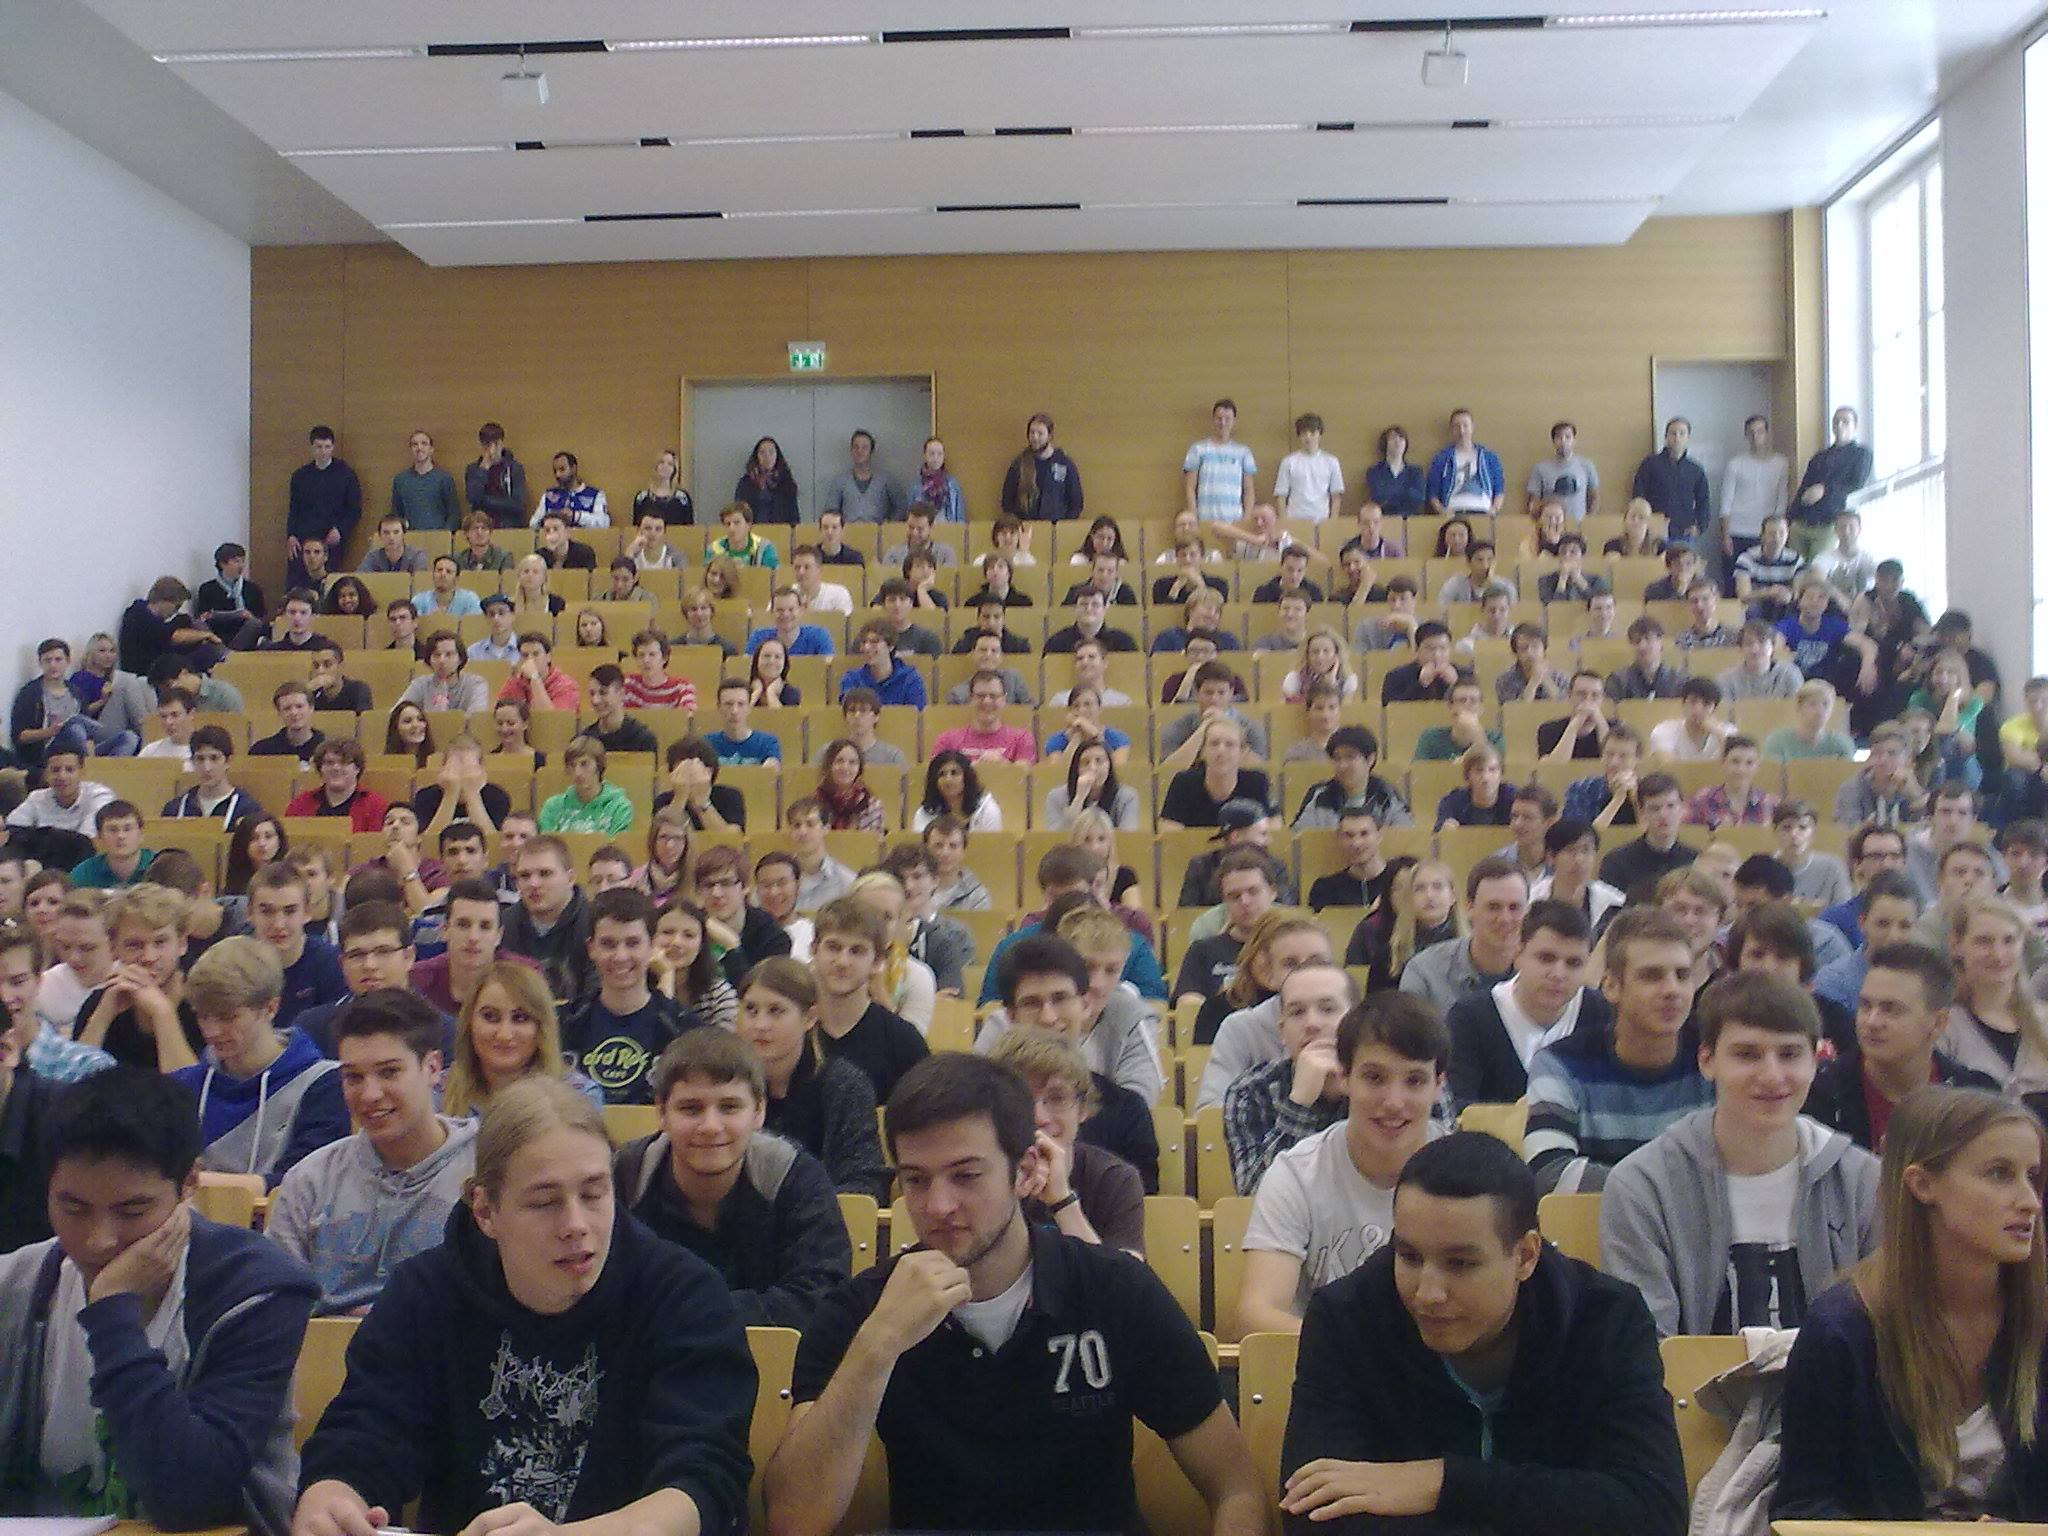
\includegraphics[scale=0.065]{ws14_15}
				\caption{WS 2013/2014}
			\end{figure}
		\end{column}
		\begin{column}{6cm}
			\begin{figure}
				\centering
				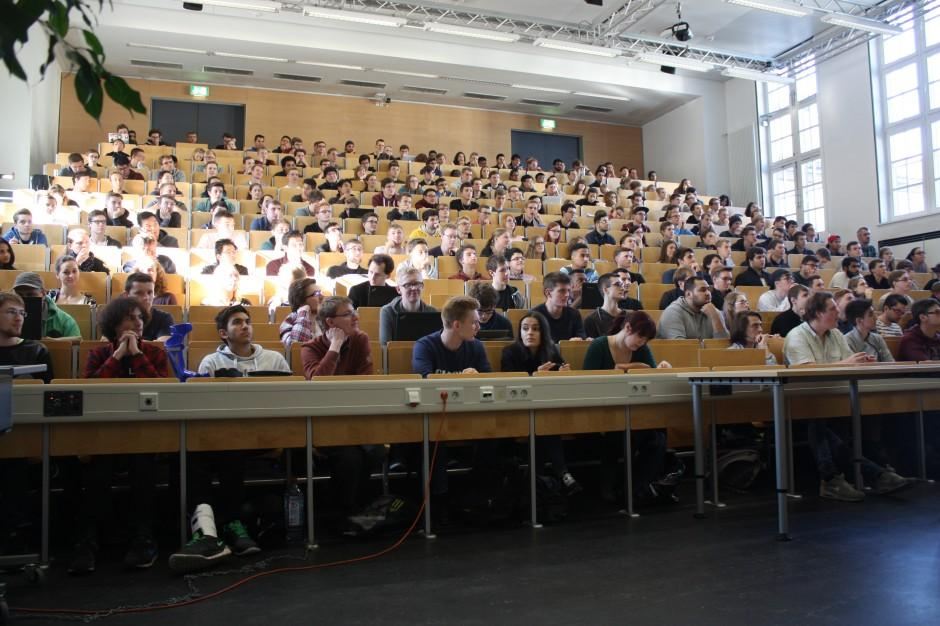
\includegraphics[scale=0.21]{ws16_17}
				\caption{WS 2016/2017}
			\end{figure}
		\end{column}
	\end{columns}}
\maketitle

\section{Vorwort}
\begin{frame}
	\slidehead
	\begin{center}
		\vspace{1cm}
		{\Huge Stream am 19.10}\\
		\vspace{1cm}
		Wenn ihr an dem Stream teilnehmen könnt und wollt, (oder daran teilgenommen habt) müsst ihr euch dieses Video nicht anschauen.\\
		Ihr müsst auch kein anderes Video bis zu diesem Stream schauen!
	\end{center}
\end{frame}

\section{Veranstalter}
\subsection*{Fachschaft Informatik}
\begin{frame}
	\slidehead
	\begin{itemize}
		\item "`Die Schüler*innenvertretung der Studierenden"'
		\item Ansprechpartner für Studierende bei Fragen zum Studium
		\item Bei Problemen zwischen Dozierenden und Studierenden vermitteln
		\item Den Studienablauf am Fachbereich weiter verbessern
		\item Soziale Interaktion zwischen Studierenden fördern
		\item Erstsemestern den Einstieg ins Studium erleichtern
		\item ...
	\end{itemize}
\centering
\vspace{3mm}
\huge Mehr auf D120.de
\end{frame}

\section{Kontakt}
\begin{frame}
	\slidehead
	\begin{itemize}
		\item \textbf{Mail:} \href{mailto:vorkurs@d120.de}{vorkurs@d120.de}
		\item \textbf{Moodle:}  \href{https://moodle.informatik.tu-darmstadt.de/course/view.php?id=624} {https://moodle.informatik.tu-darmstadt.de}
	\end{itemize}
	\vspace{2.5cm}
	\begin{alertblock}{Hinweise}
		Ihr habt allgemeine Fragen: Schreibt ins Moodle-Forum. \\
		Ihr habt spezielle Fragen an uns: Schreibt uns eine Mail. \\
		Ihr könnt uns natürlich auch in Discord ansprechen.
	\end{alertblock}
\end{frame}

\section{Ablauf des Vorkurses}
\subsection{Ein üblicher Tag im Vorkurs}
\begin{frame}
	\slidehead
	\begin{itemize}
		\item \textbf{Vormittags "`Vorlesung"' (stream)}
		\begin{itemize}
			\item interaktiv
			\item heißt: Fragen stellen
			\item Stream auf TODO LINK!
		\end{itemize}
		\item \textbf{Mittagspause}
		\begin{itemize}
			\item Pausen sind wichtig
			\item Wir können leider nicht in die Mensa :(
			\item Discord ist offen.
		\end{itemize}
		\item \textbf{Nachmittags Übung}
		\begin{itemize}
			\item Gruppenarbeit (Discord räume)
			\item Tutor*innen in Discord
			\item offenes Ende
		\end{itemize}
	\end{itemize}
\end{frame}

\subsection{Wochenplan}
\begin{frame}
	\slidehead
	\textbf{Allgemeines Programm}
	\begin{itemize}
		\item Montag
		\begin{itemize}
			\item Infostream um TODO UHRZEIT
			\item Python Installieren (Hilfe in Discord)
			\item Inhaltsstream um TODO UHRZEIT
			\item Nachmittags: Übung in Discord
		\end{itemize}
		\item Dienstag, Mittwoch, Donnerstag
		\begin{itemize}
			\item Stream um TODO UHRZEIT
			\item Nachmittags: Übung in Discord
		\end{itemize}
		\item Freitag
		\begin{itemize}
			\item Stream um TODO UHRZEIT
			\item Nachmittags: Übung in Discord
			\item Abschlusstream um TODO UHRZEIT
		\end{itemize}
	\end{itemize}
\end{frame}

\subsection{Stoffplan}
\begin{frame}
	\slidehead
	\begin{itemize}
		\item Erste schritte im Programmieren?
		\item Was ist Python?
		\item Mein erstes Programm
		\item Datentypen und Operatoren
		\item Schleifen und bedingte Anweisungen
		\item Funktionen \& Rekursion
	\end{itemize}
\end{frame}

\subsection{Voraussetzungen}
\begin{frame}
	\slidehead
	\centering
	\vspace{1.5cm}
	\tiny Ein internetfähiges Endgerät,\\ansonsten:\\
	\Huge Keine
\end{frame}

\subsection{Ziele}
\begin{frame}
	\slidehead
	\begin{itemize}
		\item Vereinfachter Start ins Studium
		\item Grundlegende Konzepte verstehen
		\item Leute Kennenlernen

	\end{itemize}
\end{frame}

\subsection{Übungsaufgaben}
\begin{frame}
	\slidehead
	\begin{itemize}
		\item Aufgaben mit unterschiedlichen Schwierigkeitsgrad
		\item Tutor*innen in Discord, die euch unterstützen
		\item Helft euch auch gegenseitig, denn so lernt ihr am meisten
		\item Ihr müsst nicht alle Aufgaben lösen
	\end{itemize}
\end{frame}

\section{Moodle}
\begin{frame}
	\slidehead
	\vskip -1.1em
	\begin{columns}
		\begin{column}{.667\linewidth}
			\begin{itemize}
				\item Vorlesungsfolien \& Übungen
				\item Ankündigungen
				\item Fragen, Foren
			\end{itemize}
		\end{column}
		\begin{column}{.3\linewidth}
			\\
			\vspace{-0.2cm}
			
\includegraphics[width=.7\linewidth]{media/moodle_qr.png}
		\end{column}
	\end{columns}
	\vspace{-0.2cm}
	\begin{block}{Lernportal Informatik - Vorkurs}
		\vskip 1 pt
		\Huge{Gastschlüssel TODO}\\
		\normalsize
		\vskip 1 pt
		Nähere Informationen zum Zugriff auf die Materialien:\\
		\quad \href{https://d120.de/vorkurs}{https://d120.de/vorkurs}
	\end{block}
\end{frame}


\section{Discord}
\begin{frame}
	\slidehead
	\vskip -1.1em
	\begin{columns}
		\begin{column}{.667\linewidth}
			\begin{itemize}
				\item Wir haben für euch einen Discord Server angelegt!
				\item dort könnt ihr euch untereinander austauschen
				\item dort könnt ihr auch mit erfahrenen Tutor*innen reden
			\end{itemize}
		\end{column}
		\begin{column}{.3\linewidth}
			\\
			\vspace{-0.2cm}
			%
\includegraphics[width=.7\linewidth]{media/moodle_qr.png} %TODO QR code für discord link
		\end{column}
	\end{columns}
	\vspace{0.9cm}
	\begin{block}{Discord - Vorkurs}
		\normalsize
		\vskip 1 pt
		Für Discord braucht ihr einen Account!\\
		Ihr könnt Discord hier herunter laden:\\
		\quad \href{https://discord.com/}{https://discord.com/}\\\\
		Mit diesen Link kommmt ihr dann auf den Server:\\
		\quad \href{TODO}{TODO}
		Lest euch bitte auf dem Server die Willkommensnachricht durch!
	\end{block}
\end{frame}


\section{YouTube}
\begin{frame}
	\slidehead
	\begin{itemize}
		\item wir streamen für euch die Vorlesungen Live
		\item ihr könnt während dessen fragen im chat stellen!
		\item Diskutiert auch gerne parallel in Discord.
	\end{itemize}
\end{frame}


\section{Ophase}
\begin{frame}
	\slidehead
	TODO
	\textbf{Nächste Woche} ist die Ophase (07. bis 11.10.2019)! \\
	Nehmt auf jeden Fall daran teil. Es lohnt sich für euch!
	\begin{figure}
		\centering
		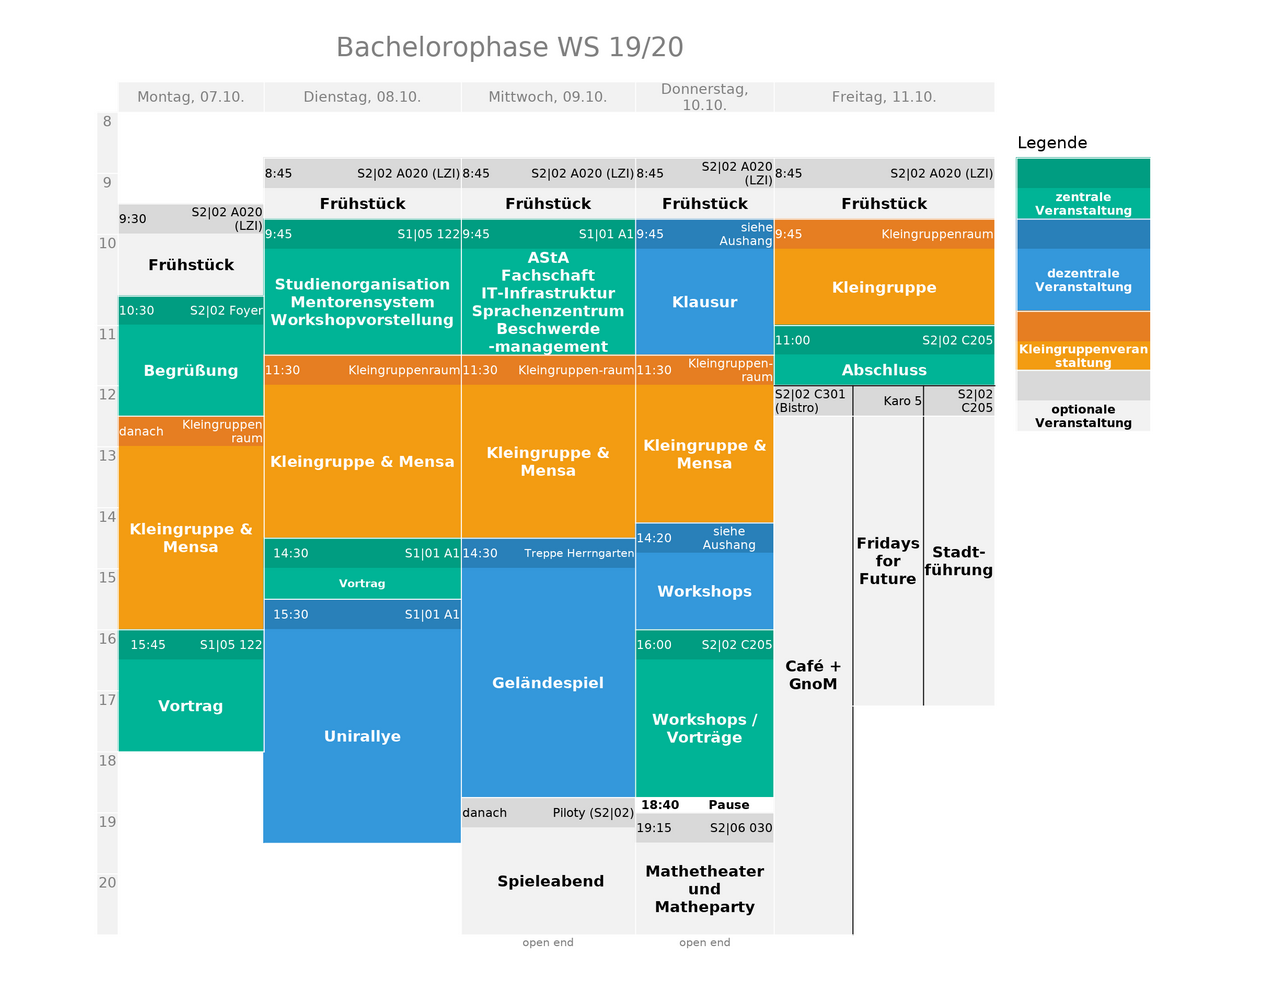
\includegraphics[scale = 0.14]{ophase}
	\end{figure}
\end{frame}

\end{document}
